\documentclass[unknownkeysallowed, final]{beamer}


\mode<presentation>
{\usetheme{I6dv}}

%\usepackage[size=custom,width=91,height=121,scale=1,debug]{beamerposter}
%\usepackage{beamerposter}
%\setlength{\paperwidth}{33.1in}
%\setlength{\paperheight}{23.4in}
%\usepackage[orientation=portrait,size=a0,scale=1.0,debug]{beamerposter}                       % e.g. for DIN-A0 poster

\setbeamerfont{itemize}{size=\normalsize}
\setbeamerfont{itemize/enumerate body}{size=\normalsize}
\setbeamerfont{itemize/enumerate subbody}{size=\normalsize}

\newtheorem{proposition}{proposition}

\DeclareMathOperator{\ch}{ch}
\DeclareMathOperator{\pa}{pa}
\DeclareMathOperator{\an}{an}
\DeclareMathOperator{\rh}{rh}
\DeclareMathOperator{\nd}{nd}

\def\ci{\perp\!\!\!\perp}
\newcommand{\E}{\mathbb{E}}

% additional packages
\usepackage{comment}
\usepackage{tikz,pgf,bm}

\usepackage[round]{natbib}
\usepackage{xcolor}

\usepackage[absolute,overlay]{textpos}

\usetikzlibrary{arrows}
\usetikzlibrary{decorations.pathreplacing}

\usepackage{times}
\usepackage{amsmath,amsthm, amssymb, latexsym}
\usepackage{exscale}
%\boldmath
\usepackage{booktabs, array}
%\usepackage{rotating} %sideways environment
\usepackage[english]{babel}
\usepackage[latin1]{inputenc}


\newcommand{\footleft}{}
\newcommand{\footright}{}

%%gets rid of bottom navigation bars
%\setbeamertemplate{footline}[frame number]{}
%
%%gets rid of bottom navigation symbols
%\setbeamertemplate{navigation symbols}{}
%
%%gets rid of footer
%%will override 'frame number' instruction above
%%comment out to revert to previous/default definitions
%\setbeamertemplate{footline}{}

\listfiles
%\graphicspath{{figures/}}

\usepackage[orientation=portrait,size=custom,width=122,height=91, scale=1.4, debug]{beamerposter}
\usepackage{color,soul}
\usepackage{float}
\usepackage{subfig}
\usepackage{multirow}

\DeclareMathOperator{\past}{past}
\DeclareMathOperator{\fix}{fix}
\DeclareMathOperator{\doo}{do}
\DeclareMathOperator{\dis}{dis}
\DeclareMathOperator{\bl}{bl}
\DeclareMathOperator{\intr}{int}
%\DeclareMathOperator{\rh}{rh}
%\DeclareMathOperator{\pa}{pa}
\DeclareMathOperator{\de}{de}
\DeclareMathOperator{\si}{si}
%\DeclareMathOperator{\ch}{ch}
%\DeclareMathOperator{\an}{an}
\DeclareMathOperator{\ancl}{ancl}
\DeclareMathOperator{\ant}{ant}
\DeclareMathOperator{\adj}{adj}
\DeclareMathOperator{\mb}{mb}
\DeclareMathOperator{\cb}{cb}
%\DeclareMathOperator{\nd}{nd}
\DeclareMathOperator{\ndp}{ndp}
\DeclareMathOperator{\nb}{nb}
\DeclareMathOperator{\fa}{fa}
\DeclareMathOperator{\sib}{sib}
\DeclareMathOperator{\pre}{pre}
\DeclareMathOperator{\tailo}{tail}
\usetikzlibrary{calc}

\title{Using Machine Learning to Improve Job Scheduling in Datacenters}

\author{Eli Sherman, Yash Kumar Lal, Brian Choi, Avais Pagarkar}
\institute{Department of Computer Science}

\begin{document}

\addtobeamertemplate{headline}{}
{\begin{tikzpicture}[remember picture,overlay] 
\node [shift={(10 cm, -3cm)}] at (current page.north west) {
\includegraphics[scale = 2]{logo2-eps-converted-to.pdf}}; 
\end{tikzpicture} }

\begin{frame}
\vspace{-1.2cm}

\begin{columns}[t]
    
%%%%%%%%%%%%%%%%%%%%%%%%%%%%%%%%%%%%%%%%%%%%%
\begin{column}{.33\linewidth}

\begin{block}{Motivation}

Background:
\begin{itemize}
        \item Scheduling algorithms within large-scale systems are necessary to manage resources and jobs.
        \begin{itemize}
            \item Shortest Job First
		    \item Dominant Resource Fairness
        \end{itemize}
\end{itemize}

\vspace{.6cm}
\alert{Problem}:  \\
    \begin{itemize}
        \item SJF-type algorithms require prior prediction of runtimes
    \end{itemize}
\vspace{.6cm}
\textcolor{blue}{Proposed Solution:} develop a machine learning-based SJF scheduling algorithm (ML-SJF), which predicts job runtimes based on the characteristics of jobs submitted to a datacenter framework
\end{block}

% \vspace{.6cm}
%++++++++++++++++++++++++++++++++++++++++++++++++
\begin{block}{Related Work}	
	\begin{itemize}
        \item Hidden markov models to predict job completion times using data extracted from supercomputing cluster logs. \cite{predictjobcompletion}
        \item Exploration of various ML techniques to model homogenous job scheduling. \cite{helmy2015machine}
        \item Fuzzy rule-based system built over job history to predict next CPU burst time \cite{fuzzycpu}
	\end{itemize}
\end{block}
%++++++++++++++++++++++++++++++++++++++++++++++++
% \begin{block}{Our Contributions}	
% 	\begin{itemize}
% 		\item Implementation of Simulated Datacenter with Mesos-like Master and Agents
% 		\item Machine-Learning Shortest Job First Scheduling Algorithm
% 		\item Empirical Comparison of ML-SJF with SJF and DRF
% 	\end{itemize}
% \end{block}
%+++++++++++++++++++++++++++++++++++++++++++++++
% \vspace{.6cm}
\begin{block}{Testbed System}
Simulate Datacenter based on Mesos Scheduling Framework
\begin{itemize}
    \item Abstraction with single master node communicating with agent node via Python sockets
    \item System receives and processes jobs
    \item Use results of job runs to train ML predictor for future job runs
\end{itemize}
\end{block}

% \vspace{.5cm}
\begin{block}{Agent Workflow}
\begin{figure}
		    \centering
		    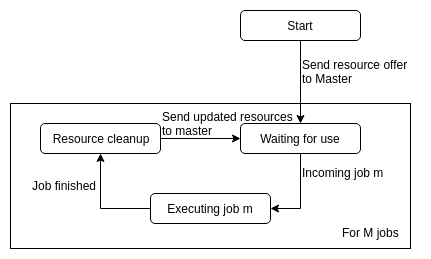
\includegraphics[height=19.5cm,width=39cm]{agent.png}
		    \caption{Agent}
		    \label{fig:agent}
		\end{figure}
\begin{itemize}
    \item Agent maintains list of resources 
    \item Executes jobs from master using os system call commands
    \item Sends updates to master when job has finished
\end{itemize}
\end{block}
%++++++++++++++++++++++++++++++++++++++++++++++++
% \begin{block}{Outline}
% 	\begin{itemize}
% 		\item Re-express ID theory in LV-DAGs concisely using \alert{kernels} and \alert{conditional graphs}
% 		\item Extend LV-DAGs to handle dependence - chain graphs (CG)
% 		\item Generalize `latent projections' to represent classes of LV-CGs that share ID theory via \alert{segregated graphs} (SG)
% 	\end{itemize}
% \end{block}
\end{column}
%++++++++++++++++++++++++++++++++++++++++++++++++
\begin{column}{.34\linewidth}

	\begin{block}{Master Workflow}
		\begin{figure}
		    \centering
		    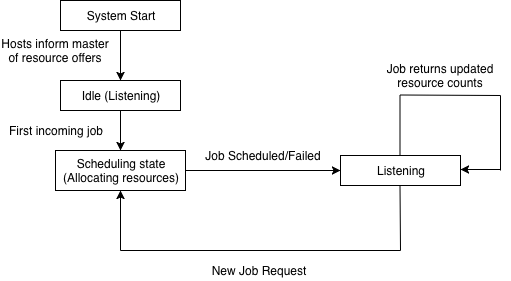
\includegraphics[height=19.5cm,width=39cm]{master.png}
		    \caption{Master}
		    \label{fig:master}
		\end{figure}
	\begin{itemize}
        \item Master maintains available resources (CPU, RAM, etc..) and list of jobs to complete
        \item Master schedules job requests of varying types (Flask, M/R, etc..) 
        \item Sends jobs to run on agents after scheduling
    \end{itemize}
\end{block}
%%%%%%%%%%%%%%%%%%%%%%%%%%%%%%%%%%%%%%%%%%%%
\vspace{.5cm}
\begin{block}{Types of Jobs}
\textbf{Web-Based}
\begin{itemize}
    \item Flask Jobs: Insertion Sort, Bubble Sort, Bogo Sort, etc...
\end{itemize}
\vspace{.3cm}
\textbf{Machine Learning Jobs}
\begin{itemize}
    \item scikit-learn Jobs: Pre-installed Datasets
\end{itemize}
\vspace{.3cm}
\textbf{Distributed Computation}
\begin{itemize}
    \item Map Reduce Jobs: Word Count on Book Excerpts
\end{itemize}
\end{block}

%%%%%%%%%%%%%%%%%%%%%%%%%%%%%%%%%%%%%%%%%%%%%%
\vspace{.5cm}
\begin{block}{Machine Learning}
\textbf{Overall Idea}
\begin{itemize}
    \item Generate 1000 jobs of each type with random features
    \item Run jobs in Mesos system to collect runtimes
    \item Train ML model
    \item Use ML model to predict future job runtimes
\end{itemize}
\vspace{.2cm}
\textbf{Input Features}
    \begin{itemize}
        \item Web-Based: size of work file, type of operation (sorting algorithm)
        \item ML Jobs: number of rows and columns in training set, number of target classes
        \item MapReduce Jobs: size of work files, number mappers, number reducers
    \end{itemize}
\vspace{.2cm}
\textbf{Model Learning}
    \begin{itemize}
        \item Support Vector Regression (SVR) is highly flexible ML algorithm
        \item Capable of learning relationships in high dimensional data
        \item Train each regressor with 5-fold CV on input data, keep best regularization parameter
    \end{itemize}
\end{block}
%++++++++++++++++++++++++++++++++++++++++++++++++


\end{column}
%%%%%%%%%%%%%%%%%%%%%%%%%%%%%%%%%%%%%%%%%%%%%%%
%++++++++++++++++++++++++++++++++++++++++++++++++
\begin{column}{.29\linewidth}
%%%%%%%%%%%%%%%%%%%%%%%%%%%%%%%%%%%%%%%%%%%%%
\begin{block}{Experiments}	
\begin{itemize}
	\item Generate additional 600 random jobs as test set
	\item Comparison of all scheduling algorithms
	\begin{itemize}
		\item Schedule jobs in test set using different algorithms and execute
		\item Log throughput and average waiting time
	\end{itemize}
	\item Analysis of runtime trends for each framework
	\begin{itemize}
	    \item Replace randomly generated predicted runtimes for test jobs with average runtime of that framework's job
	    \item Schedule each framework's jobs using SJF and execute
	    \item Log throughput and average waiting time
	\end{itemize}
\end{itemize}
\end{block}
%+++++++++++++++++++++++++++++++++++++++
\vspace{.16cm}
\begin{block}{Results (Experiment 1)}

\begin{table}[!tbh]
\centering
\begin{tabular}{|c|c|c|}
    \hline
    \textbf{Algorithm} & \textbf{Throughput} & \textbf{Avg Wait Time} \\\hline
    DRF & 0.3522 & 835.95 secs \\\hline
    SJF & 0.4735 & 643.31 secs \\\hline
    ML-SJF & 0.1561 & 1713.26 secs \\\hline
    Hard-coded & 0.1689 & 1734.43 secs \\\hline
\end{tabular}
\caption{Performance of algorithms overall}
\label{all-jobs}
\end{table}
\begin{itemize}
	\item ML-SJF has a lower throughput than the conventional SJF and DRF implementations, contrary to our hypothesis.
	\item In ML-SJF, the three types of jobs generally are in three different ranges of runtime
	\item MapReduce jobs are almost always executed in parallel with other MapReduce jobs in case of ML-SJF, reducing the throughput. 
\end{itemize}
\vspace{-.4cm}
\end{block}

\vspace{.16cm}
\begin{block}{Results (Experiment 2)}

\begin{table}[h]
\begin{tabular}{|c|c|c|c|}
\hline
    \textbf{Job type} & \textbf{Algorithm} & \textbf{Throughput} & \textbf{Avg Wait Time} \\\hline
    MR & SJF & 0.1371 & 310.875 secs \\\hline
    MR & ML-SJF & 0.1375 & 273.97 secs \\\hline
    ML & SJF & 0.1675 & 897.045 secs \\\hline
    ML & ML-SJF & 0.3324 & 437.83 secs \\\hline
    Flask & SJF & 0.1494  & 568.78 secs \\\hline
    Flask & ML-SJF & 0.1393  & 554.29 secs \\\hline
\end{tabular}
\caption{Performance of algorithms with one framework}
\label{individual-jobs}
\end{table}
\begin{itemize}
	\item For homogeneous jobs,ML-SJF outperforms SJF
	\item This is due to SJF not having the advantage of scheduling different types of jobs together.
\end{itemize}
\vspace{-.4cm}
\end{block}

\vspace{.16cm}
\begin{block}{References}

\bibliographystyle{plainnat}
\scriptsize\bibliography{bibliography.bib}

\end{block}


\end{column}

%%%%%%%%%%%%%%%%%%%%%%%%%%%%%%%%%%%%%%%%%%%%%%%

\end{columns}
\end{frame}

\end{document}
